\documentclass[11pt,letterpaper]{article}
\usepackage[latin1]{inputenc}
\usepackage[left=3.00cm, right=3.00cm, top=3.00cm, bottom=3.00cm]{geometry}
\usepackage{amsmath}
\usepackage{amsthm}
\usepackage{fancyhdr}
\pagestyle{fancy}

\usepackage{mathtools}
\DeclarePairedDelimiter\ceil{\lceil}{\rceil}
\DeclarePairedDelimiter\floor{\lfloor}{\rfloor}

\usepackage{color}
\usepackage{listings}
\usepackage{caption}

\usepackage{graphicx}

\newcounter{nalg}[section] % defines algorithm counter for chapter-level
\renewcommand{\thenalg}{\thechapter .\arabic{nalg}} %defines appearance of the algorithm counter
\DeclareCaptionLabelFormat{algocaption}{Algorithm \thenalg} % defines a new caption label as Algorithm x.y

\lstnewenvironment{algorithm}[1][] %defines the algorithm listing environment
{   
    \refstepcounter{nalg} %increments algorithm number
    \captionsetup{labelformat=algocaption,labelsep=colon} %defines the caption setup for: it uses label format as the declared caption label above and makes label and caption text to be separated by a ':'
    \lstset{ %this is the stype
        mathescape=true,
        frame=tB,
        numbers=left, 
        numberstyle=\tiny,
        basicstyle=\scriptsize, 
        keywordstyle=\color{blue}\bfseries\em,
        keywords={,input, output, return, datatype, function, in, if, else, foreach, while, begin, end, true, false, int, for, then, } %add the keywords you want, or load a language as Rubens explains in his comment above.
        numbers=left,
        xleftmargin=.02\textwidth,
        #1 % this is to add specific settings to an usage of this environment (for instnce, the caption and referable label)
    }
}
{}

\author{Simon Zheng\\260744353}
\title{Homework 1}
\date{September 22$^{\textnormal{nd}}$, 2017}
\lhead{COMP 251}
\rhead{Algorithms and Data Structures}

\begin{document}
	\maketitle
	\thispagestyle{fancy}
	
	\section{Stable marriage matching problem}
	
		\paragraph{a)}
		\begin{align*}
		m_1 : w_1 , w_2 , w_3 , w_4 \\
		m_2 : w_2 , w_1 , w_3 , w_4 \\
		m_3 : w_3 , w_2 , w_1 , w_4 \\
		m_4 : w_4 , w_2 , w_3 , w_1 \\
		w_1 : w_4 , w_2 , w_3 , w_1 \\
		w_2 : w_1 , w_4 , w_3 , w_2 \\
		w_3 : w_1 , w_2 , w_4 , w_3 \\
		w_4 : w_1 , w_2 , w_3 , w_4 \\
		\end{align*}
    
    Simply assume each man has a different woman as first choice (and they are respectively the worst choice of the woman). Since the algorithm is ran on the men, each proposes to their first choice one after the other and the women must accept. The men also do not break up any pairings as they are all different. The algorithm terminates, so the rest doesn't even matter.
		
		\paragraph{b)}
		.
		
		\paragraph{c)}
		\begin{center}
		Algorithm: f()
		\end{center}
		\begin{algorithm}[caption={}, label={alg2}]
Input: 
Output: 


		\end{algorithm}
		
		\paragraph{d)}
		
		
	\section{}
	
		\paragraph{a)}
		.
		\begin{center}
		Algorithm: f()
		\end{center}
		\begin{algorithm}[caption={}, label={alg3}]
Input: 
Output: 


		\end{algorithm}
		
		\paragraph{b)}
		.
		
	\section{}
	
		\paragraph{a)}
		\begin{figure}[h]
			\centering
			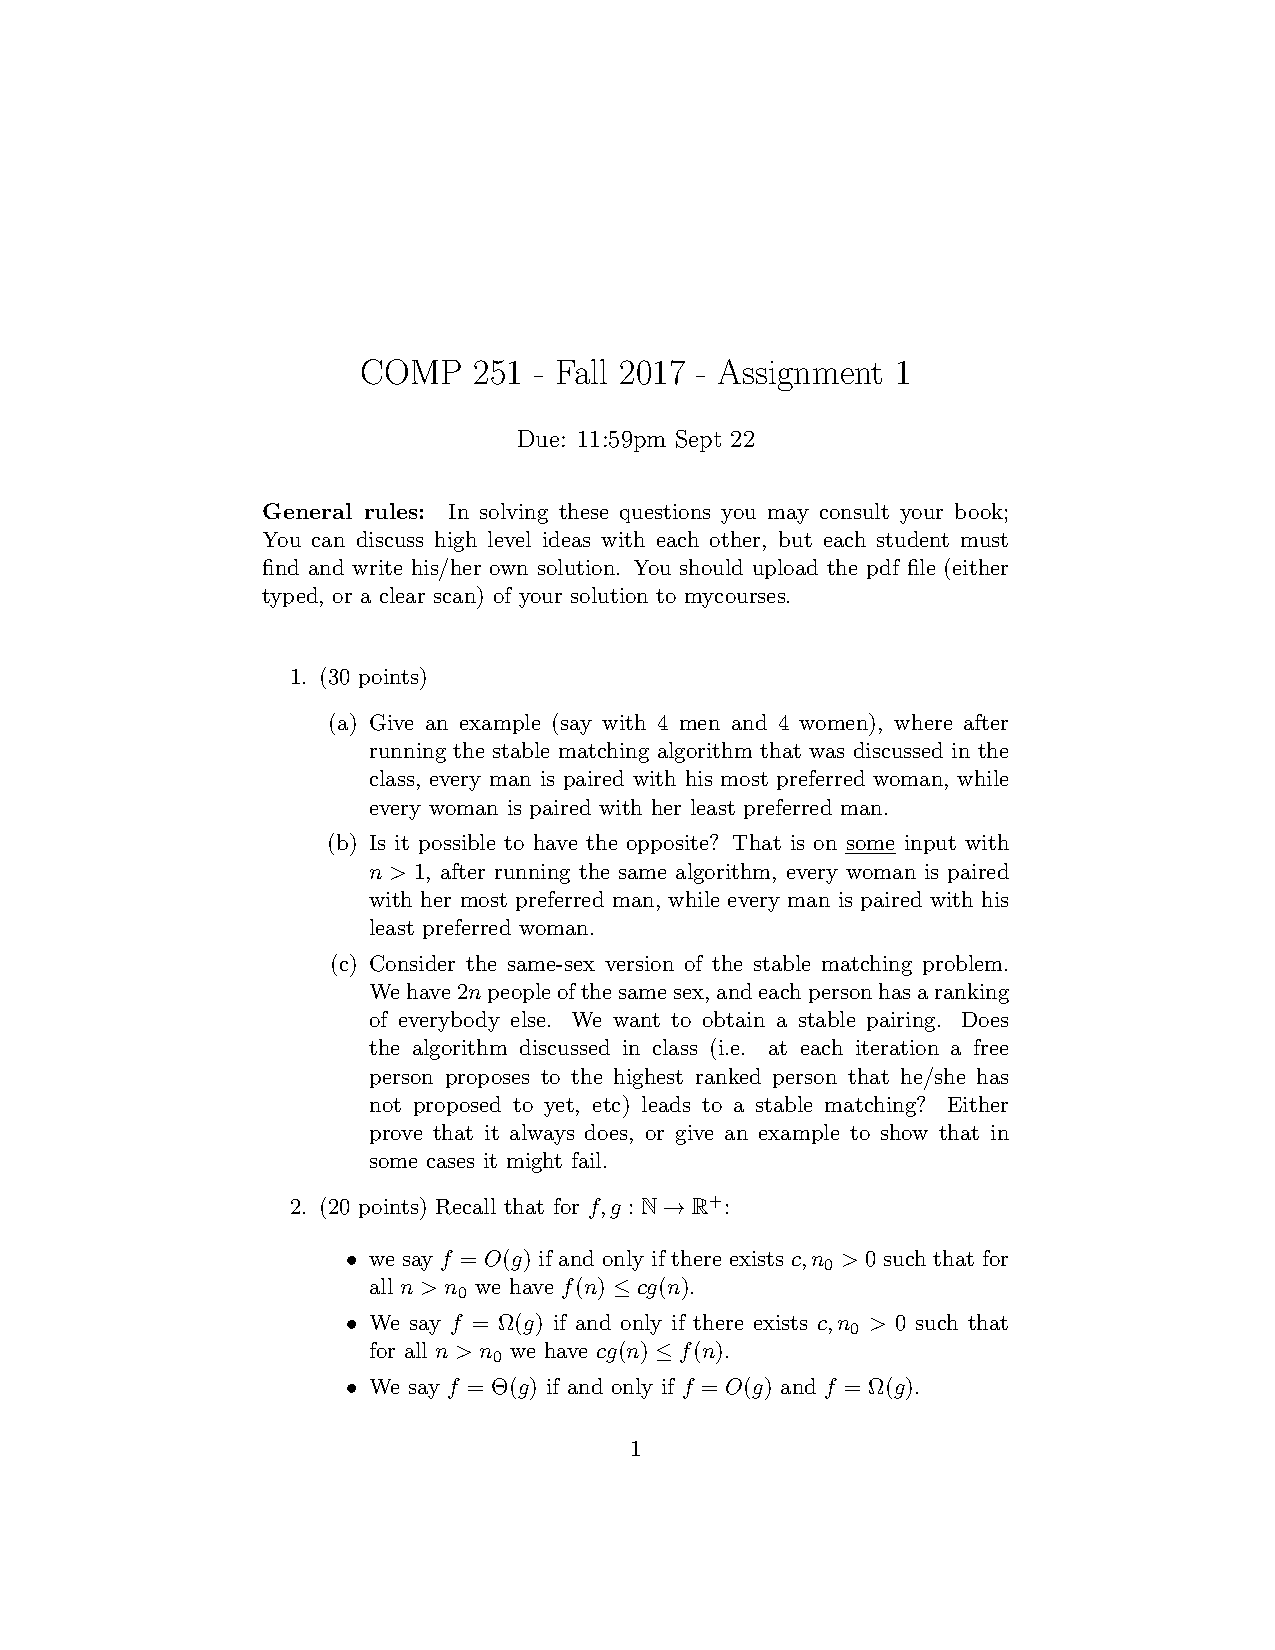
\includegraphics[width=\textwidth]{hw1.pdf}
		\end{figure}
	.
		
		\paragraph{b)}
		.
		
	\section{}
	
		\paragraph{a)}
		.
		\begin{algorithm}[caption={f()}, label={alg4}]
Input: 
Output: 


		\end{algorithm}
		
		\paragraph{b)}
		.
		
		\begin{algorithm}[caption={f()}, label={alg5}]
Input: 
Output: 


		\end{algorithm}
		
\end{document}
